\subsection{Restrições operativas do sistema}

O problema de reconfiguração está sujeita a restrições operativas imposta pela agência reguladora, tais como limite de tensão, correntes tanto para o conjunto de ramos do sistema quanto para a operação das chaves.
Dessa forma é possível determinar as restrições operativas para o funcionamento do SDEE.

\subsubsection{Limites de tensão}

Em um sistema de distribuição de energia elétrica é preciso garantir que a tensão em um nó esteja dentro de uma faixa de operação determinada por norma, por isso uma restrição fundamental para o problema é a restrição de limites de tensão em um nó, determinada pela seguinte equação:

\begin{equation}
    \underline{V}^{2} \leq V_{i}^{sqr} \leq \overline{V}^{2}\qquad\forall i \in\Omega_{b}
\end{equation}

Onde $\underline{V}$ e $\overline{V}$ representam o limite inferior e superior de tensão, respectivamente, que uma rede pode possuir.


\subsubsection{Limite de corrente}

Assim como as tensões, o fluxo de corrente também deve ser limitado para não comprometer o SDEE.
Assim a equação que descreve a restrição é:

\begin{equation}
    0 \leq I_{ij}^{sqr} \leq \overline{I}_{ij}^{2} \qquad\forall ij\in\Omega_{l} 
\end{equation}

\subsubsection{Chaves presentes no sistema}

Para reconfiguração do SDEE, existem chaves ao longo da rede que podem ser modificadas de modo a garantir a operação desejada.
Considere as seguintes restrições:

\begin{figure}[H]
    \centering
    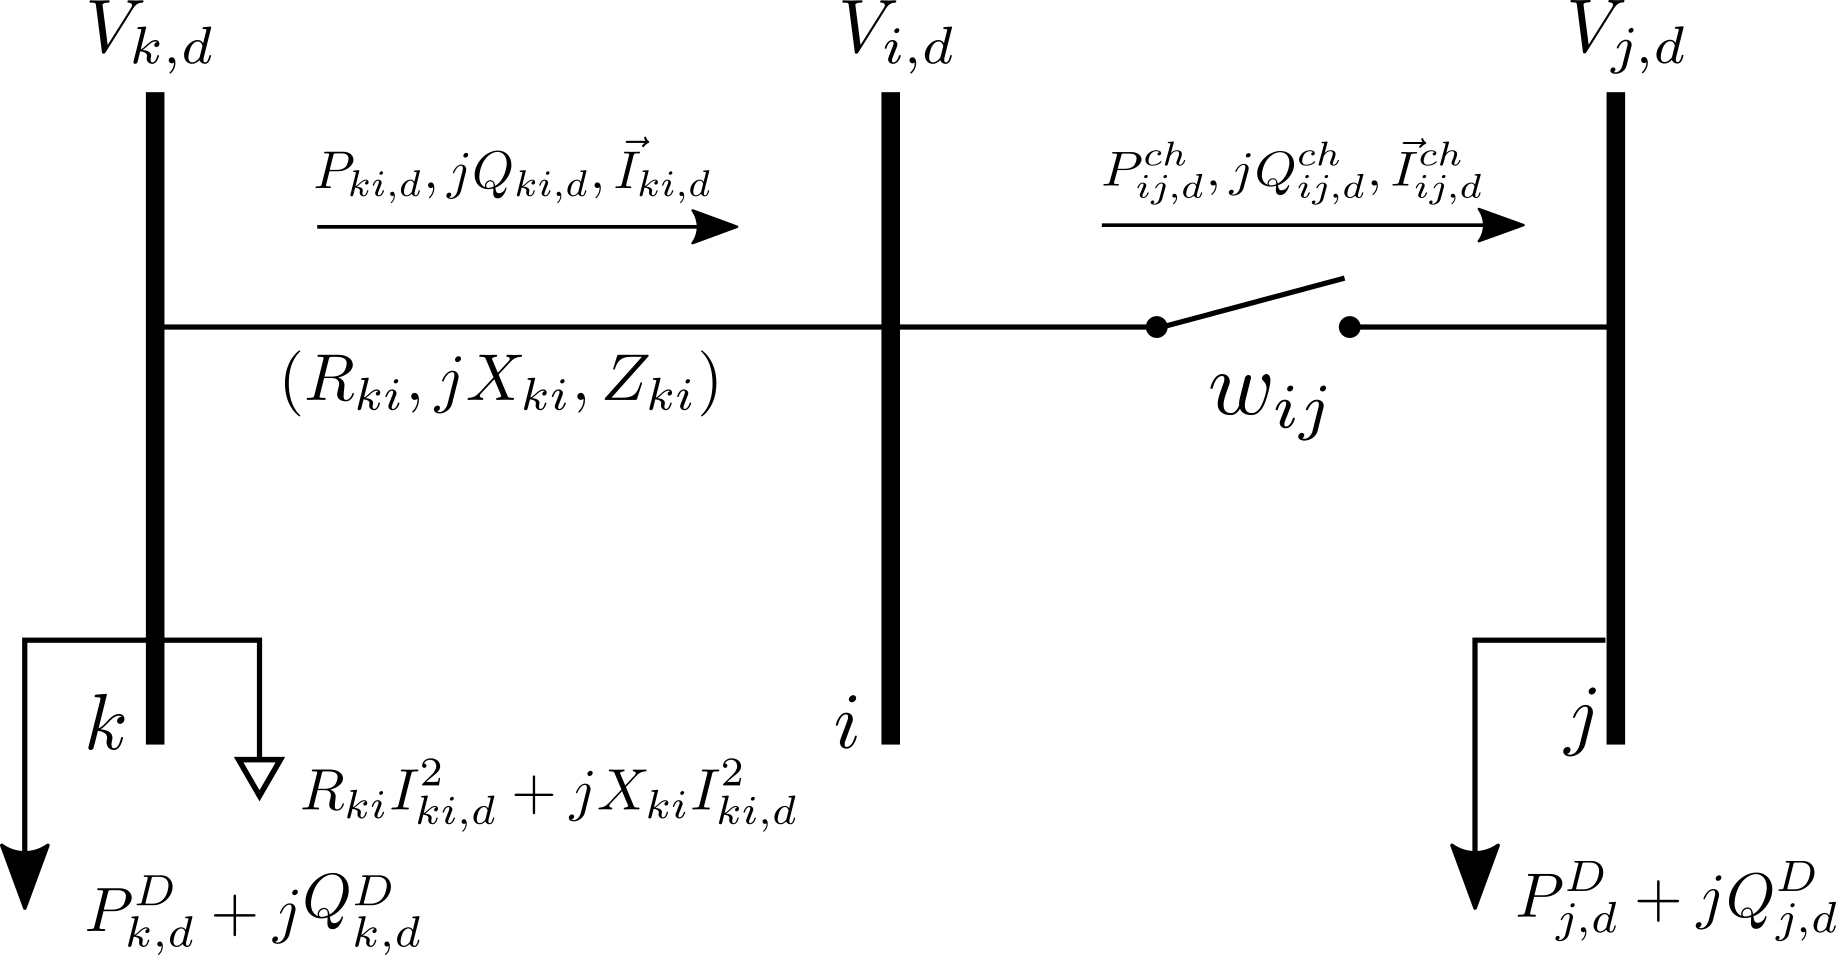
\includegraphics[scale = 1.3]{4_Modeling/diagrama_chaves.png}
    \caption{Modelo de uma chave conectada entre dois nós}
    \label{fig:diagrama_chave}
\end{figure}
    
\begin{itemize}
    \item Balanço de potência
\end{itemize}
    Com base na figura \eqref{fig:diagrama_chave}, faz-se necessário reformular as equações de balanço de potência, expressas em~\eqref{eq:fluxo_pot_ativa} e \eqref{eq:fluxo_pot_reativa}, adicionando as variáveis que representam as chaves na modelagem do problema.

\begin{equation}
    \sum_{ji\in\Omega_{l}}P_{ji} - \sum_{ij\in\Omega_{l}}(P_{ij} + R_{ij}I_{ij}^{sqr})+ \sum_{ji\in\Omega_{ch}}P_{ji}^{ch} -\sum_{ij\in\Omega_{ch}}P_{ij}^{ch} + P_{i}^{S} = P_{i}^{D}\quad\forall i \in\Omega_{b}\label{eq:fluxo_pot_ativa_chaves}  
\end{equation}
    
    
\begin{equation}
    \sum_{ji\in\Omega_{l}}Q_{ji} - \sum_{ij\in\Omega_{l}}(Q_{ij} + X_{ij}I_{ij}^{sqr})+ \sum_{ji\in\Omega_{ch}}Q_{ji}^{ch} -\sum_{ij\in\Omega_{ch}}Q_{ij}^{ch} + Q_{i}^{S} = P_{i}^{D}\quad\forall i \in\Omega_{b}
    \label{eq:fluxo_pot_reativa_chaves}
\end{equation}
    
Onde $\Omega_{ch}$ representa o conjunto de chaves da rede elétrica e $w_{ij}$ é uma variável binária que representa o estado da chave \textit{ij}: se $w_{ij} = 1$ a chave ij está fechada, caso contrário a chave está aberta, ver figura~\ref{fig:diagrama_chave}. $P_{ij}^{ch}$ e $Q_{ij}^{ch}$ representam o fluxo de potência ativa e reativa da chave \textit{ij}.

As restrições expressas nas equações \eqref{eq:fluxo_pot_ativa_chaves} e \eqref{eq:fluxo_pot_reativa_chaves} são extensões das equações \eqref{eq:fluxo_pot_ativa} e \eqref{eq:fluxo_pot_reativa}, considerando a presença de chaves na rede elétrica.
    
Além do balanço de potência, outras restrições devem ser estabelecidas devido à presença de chaves, são elas:

\begin{itemize}
    \item Diferença de tensões entre dois nós conectados por uma chave
\end{itemize}

    
A diferença de tensão entre nós, na presença de chaves, deve ser igual a zero, uma vez que, de acordo com as hipóteses adotadas, a impedância da chaves é representada como uma impedância nula.
Sendo assim, usando a variável binária $w_{ij}$ é possível equacionar a restrição da seguinte forma:

\begin{equation}
    -(\overline{V}^{2} - \underline{V}^{2})(1-w_{ij}) \leq V_{i}^{sqr} - V_{j}^{sqr} \leq (\overline{V}^{2} - \underline{V}^{2})(1-w_{ij})\qquad\forall ij\in\Omega_{ch}
\end{equation}
    
É possível observar que se $w_{ij}$ for igual a 1 (chave fechada), a diferença entre as tensões no nó $i$ e nó $j$ será igual a zero, o que condiz a hipótese adotada.

\begin{itemize}
   \item Fluxo de potência na chave
\end{itemize} 
    
O fluxo de potência na chave é determinada pelas equações abaixo.
    
\begin{equation}
    -(\overline{V}\,\overline{I}_{ij}^{ch})w_{ij} \leq P_{ij}^{ch} \leq (\overline{V}\,\overline{I}_{ij}^{ch})w_{ij}\qquad\forall ij\in\Omega_{ch}   
\end{equation}
    
    
\begin{equation}
    -(\overline{V}\,\overline{I}_{ij}^{ch})w_{ij} \leq Q_{ij}^{ch} \leq (\overline{V}\,\overline{I}_{ij}^{ch})w_{ij}\qquad\forall ij\in\Omega_{ch}   
\end{equation}
    
É possível notar que se a variável $w_{ij}$ for igual a 0 (chave aberta), o fluxo de potência na chave é igual a zero, o que condiz com a proposta do elemento de circuito na rede; quando igual a 1, as restrições representam o fluxo máximo de potência ativa e reativa permitida na chave quando está energizada.

\subsubsection{Restrição de radialidade}

A representação de um SDEE é feita através de nós e circuitos. Fazendo analogia com a teoria de grafos, um SDEE pode ser considerado como um grafo formado por n arcos e m nós.
Da teoria de grafos, uma árvore é um grafo conexo sem ciclos, assim é possível comparar a topologia radial de um SDEE com uma árvore.
Como mostrado em \cite{Bazaraa1990LinearFlows}, a árvore de um grafo é um sub-grafo com ($m-1$) arcos.

Assim, pode-se dizer que a topologia de um SDEE com $n_{b}$ nós é radial se satisfaz as duas seguintes condições: Condição 1: a solução deve apresentar ($n_{b}$) circuitos; e Condição 2: a solução deve gerar uma topologia conexa. Observa-se que a restrição de radialidade tem que ser formada pelas condições 1 e 2.
Somente a condição 1 não garante a radialidade do SDEE. 

O problema de RSD cumpre com as seguintes características: 1) apenas uma única subestação existente no SDEE (nó da subestação); 2) todos os outros nós são nós de carga; 3) a primeira lei de kirchhoff, deve ser cumprida, e 4) o objetivo é encontrar a melhor topologia radial. 
A condição 1 é satisfeita pela seguinte restrição:

\begin{equation}
    |\Omega_{l}| + \sum_{ij\in\Omega_{ch}}w_{ij} = |\Omega_{b}| - 1
    \label{eq:radialidade}
\end{equation}

Em que $|\Omega|$ é um operador que calcula o número de elementos do conjunto $\Omega$.

Uma solução que satisfaz a restrição de balanço de potência (primeira Lei de Kirchhoff) tem de fornecer a demanda de potência em cada nó de carga de modo que exista um caminho entre a subestação e os nós de carga. Portanto, cada nó está ligado com a subestação, formando um grafo conexo, o que comprova a Condição 2. 
Assim, quando as restrições de balanço de potência são combinadas com a Condição 1, cada nó de carga está ligado por um único caminho com a subestação, isto é, o SDEE é conexo, sem malhas.

\begin{figure}[H]
    \centering
    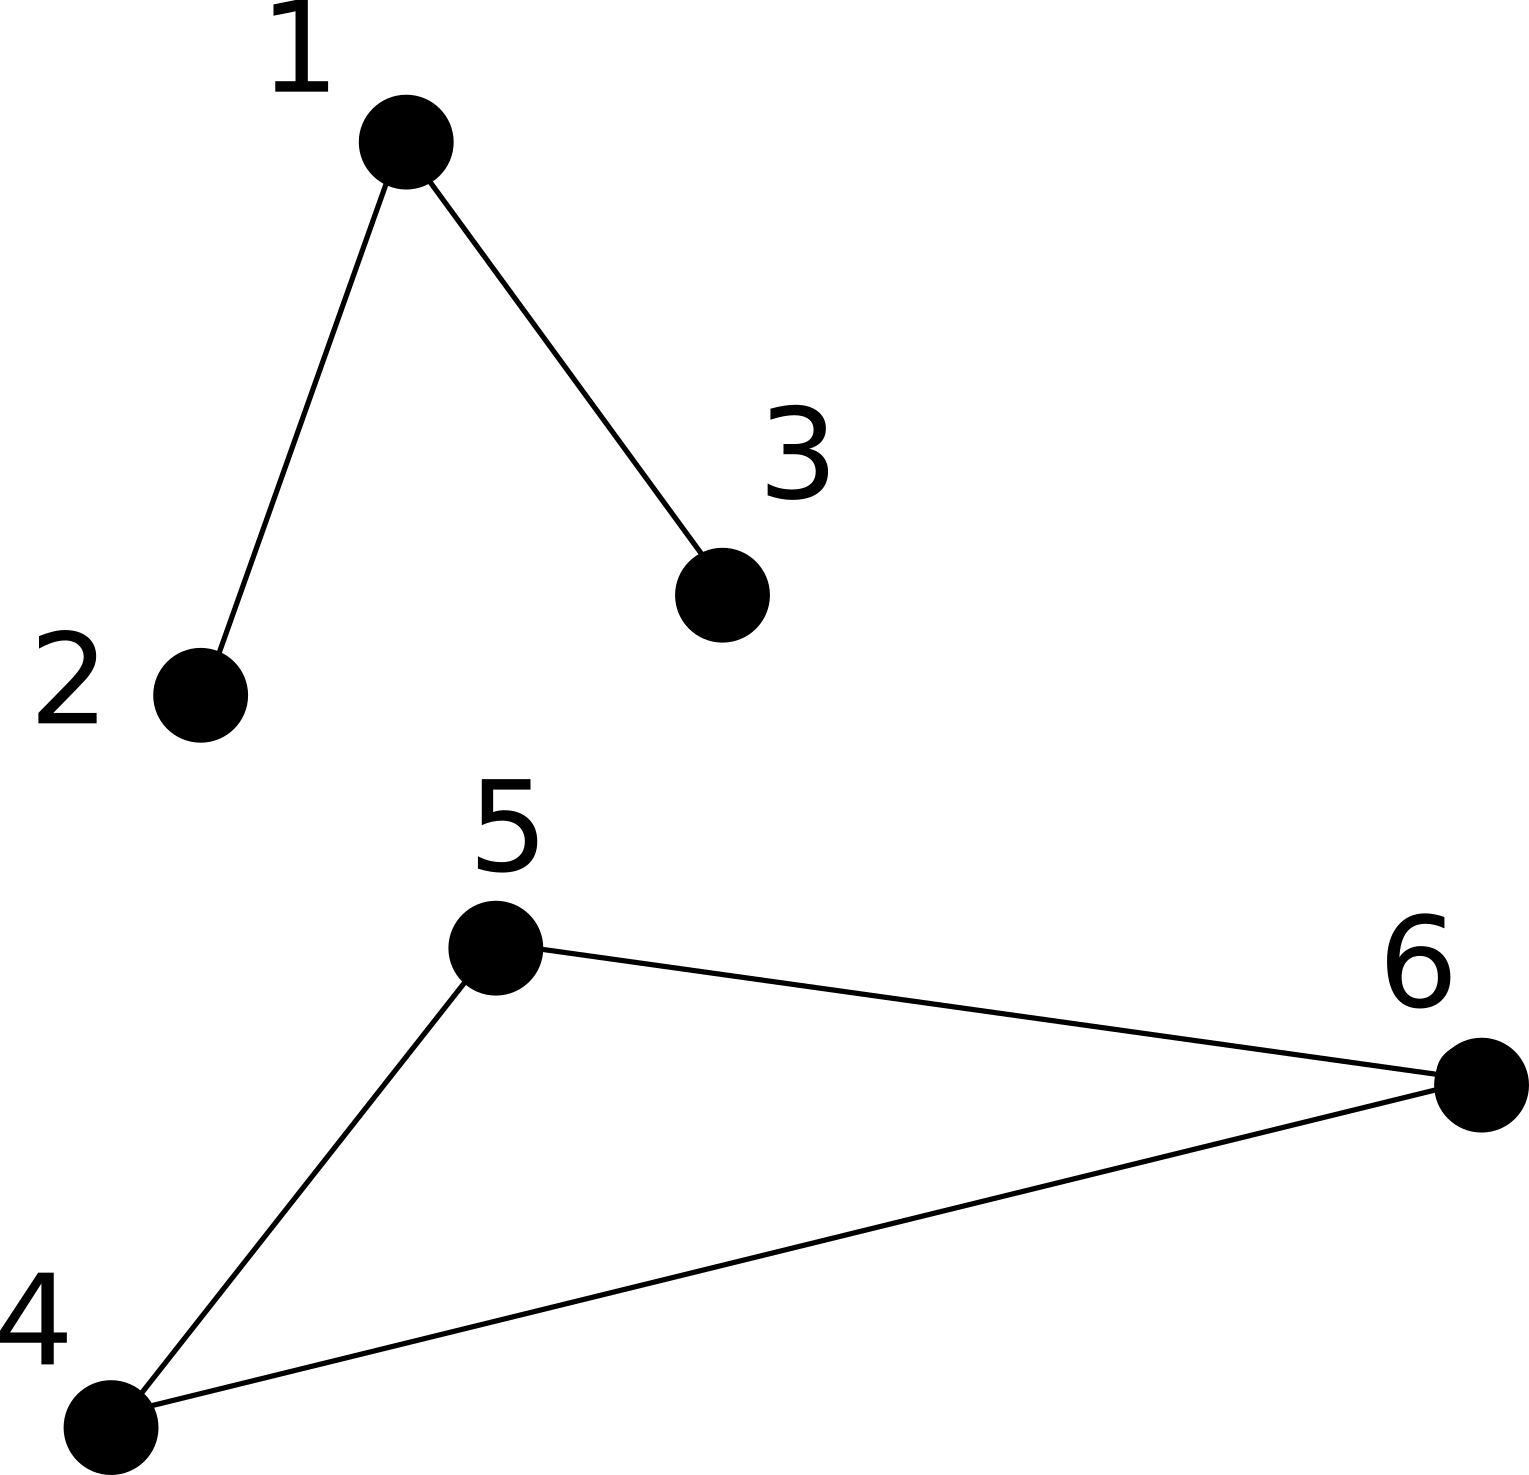
\includegraphics[scale = 0.8]{4_Modeling/restricao_fail.png}
    \caption{Exemplo de rede não radial que obedece a equação \eqref{eq:radialidade}}
    \label{fig:radialidade_wrong}
\end{figure}

Observa-se que a figura \ref{fig:radialidade_wrong}, embora respeite a equação \eqref{eq:radialidade} (5 ramos para 6 nós), não é uma topologia radial. Isso pode acontecer se e somente se a equação~\eqref{eq:radialidade} for levada em consideração.

\begin{figure}[H]
    \centering
    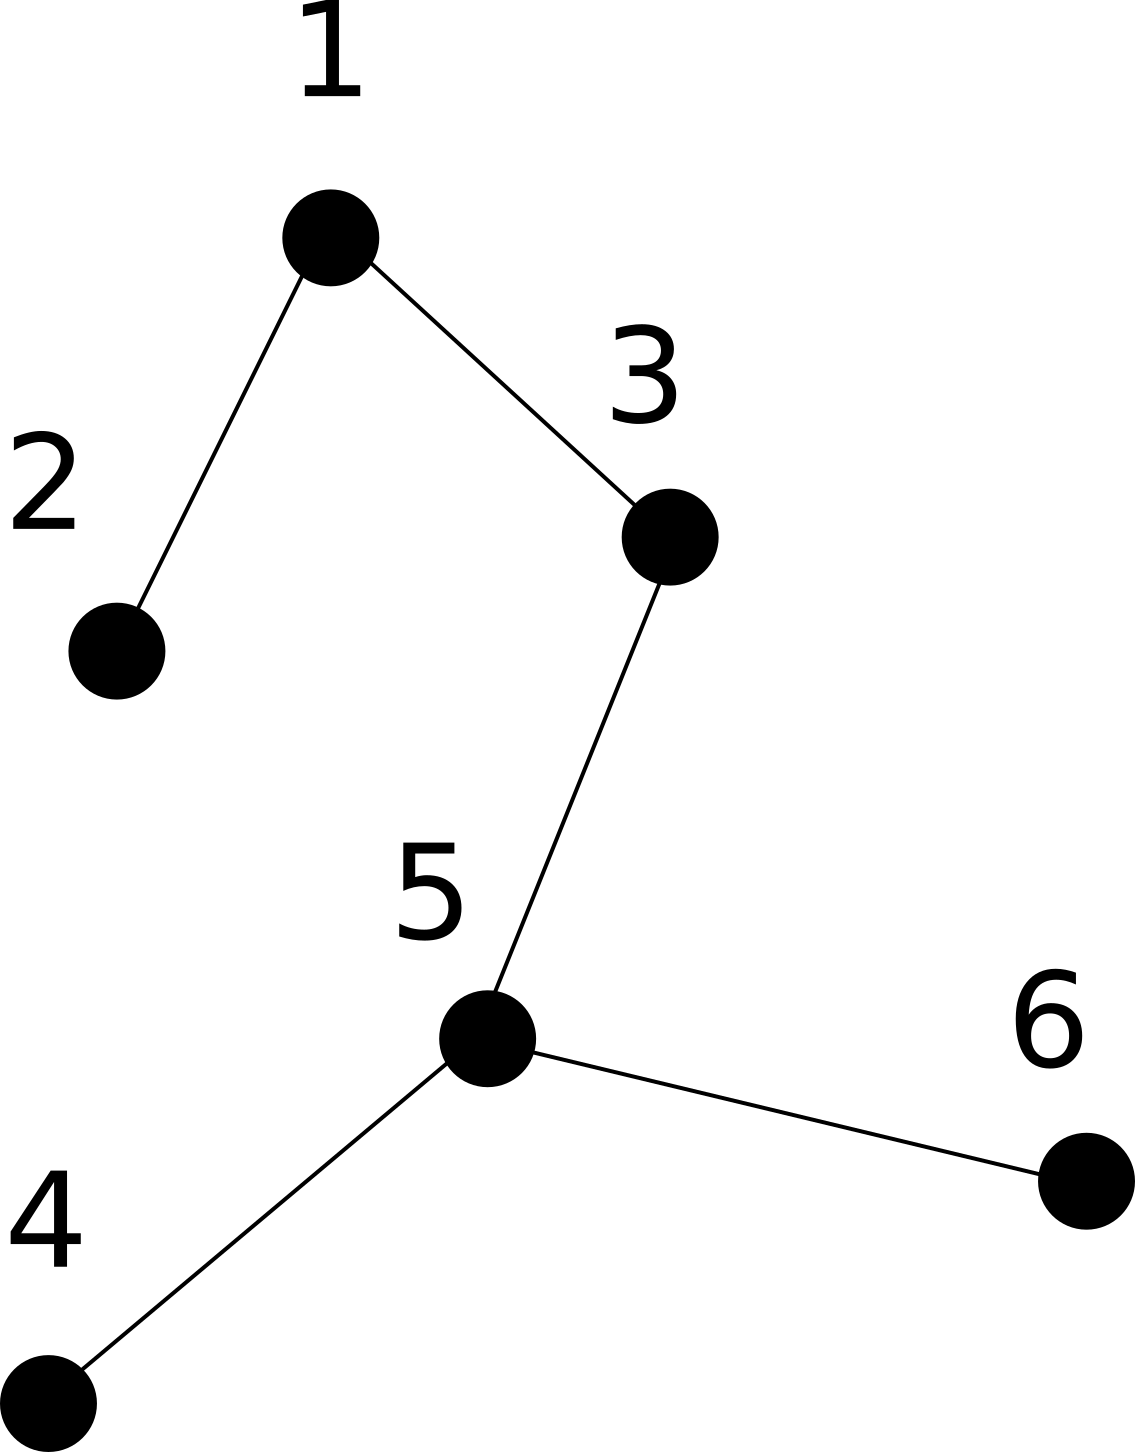
\includegraphics[scale=0.6]{4_Modeling/restricao_radialidade.png}
    \caption{Exemplo de rede radial que obedece a equação \eqref{eq:radialidade}}
    \label{fig:radialidade_right}
\end{figure}

Observe agora a figura \ref{fig:radialidade_right}, note que ela é uma topologia radial, como dito anteriormente é necessário duas condições para garantir tal configuração, como no problema já existem equações que garantem a primeira Lei de Kirchhoff, a topologia final será radial. 
É possível notar que todos os nós estão interligados, direto e não direto, com o nó 1 (nó da subestação).
Isso acontece pois as equações de balanço de potência obrigam que haja fluxo de potência para atender as demandas dos mesmos.

Assim a equação \eqref{eq:radialidade} junto com \eqref{eq:fluxo_pot_ativa_chaves} e \eqref{eq:fluxo_pot_reativa_chaves} fornecem as condições necessárias para e suficientes para garantir uma topologia final radial \cite{Lavorato2012ImposingProblems}.

